\subsection{SDK}

\subsubsection{Creazione di un widget immagine}

\label{Creazione di un widget immagine}
\begin{figure}[ht]
	\centering
	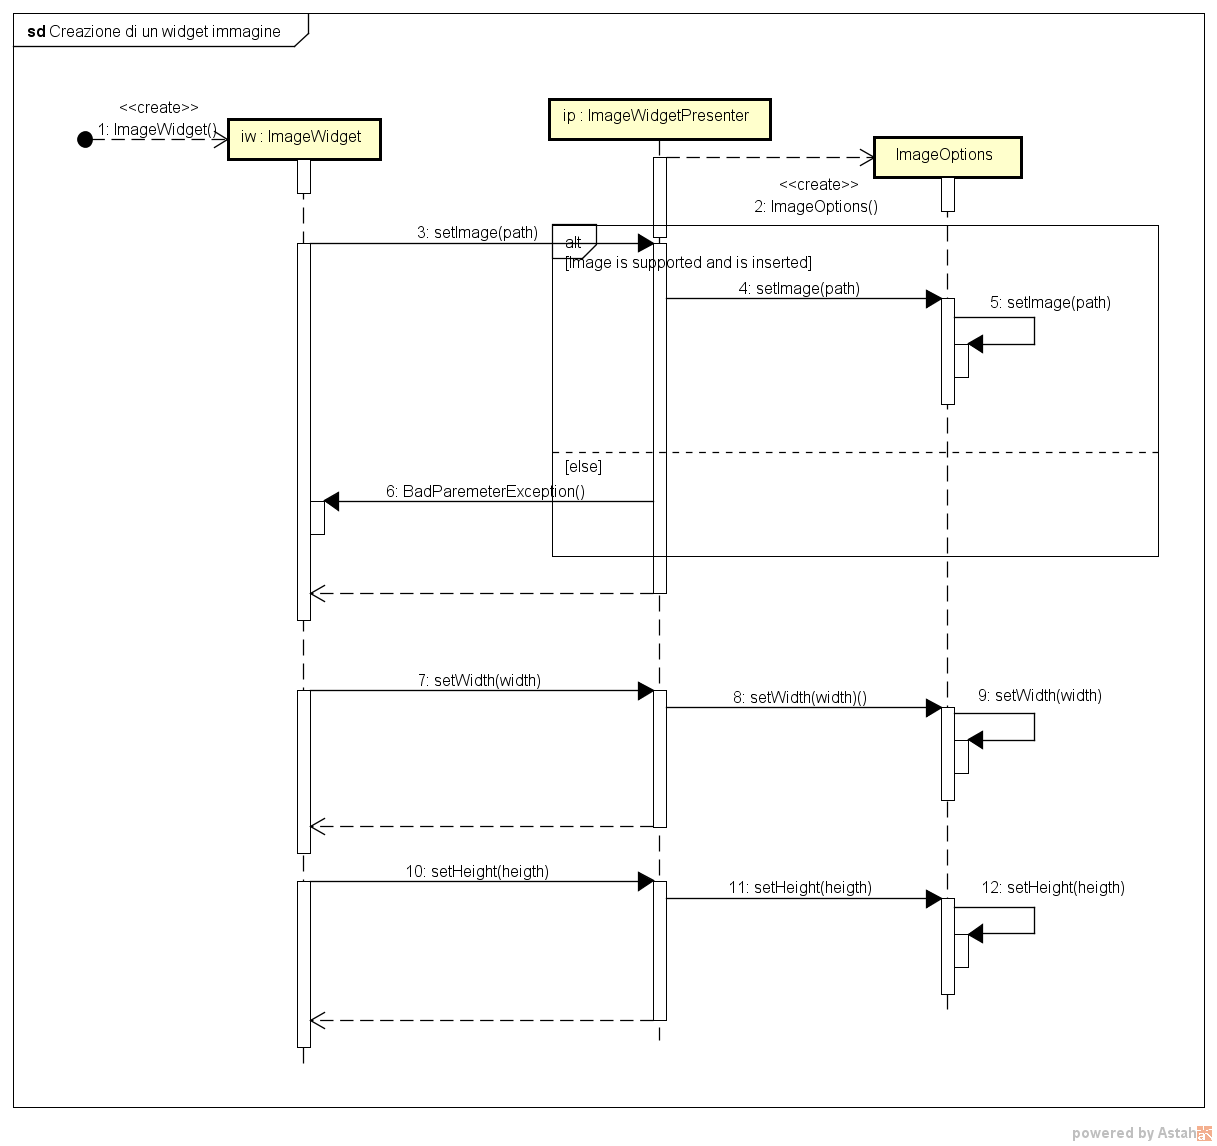
\includegraphics[width=16cm, height=14cm]{Sezioni/Diagrammi/SDK/Creazione di un widget immagine.png}
	\caption{Creazione di un widget immagine}
\end{figure}

Lo sviluppatore può creare un widget di tipo immagine per aggiungerlo ad una sua ipotetica \termine{bolla}. Durante la costruzione, come si vede dallo schema, vengono invocati tre metodi. Il primo per impostare l'immagine e gli altri due per impostare rispettivamente la larghezza ed altezza di essa. Il tipo delle immagini supportate sono le stesse supportate da \termine{Rocket.Chat} ovvero:
\begin{itemize}
\item .jpeg
\item .gif
\item .png
\item .jpg
\end{itemize}
Se l'immagine inserita non appartiene ad uno di questi formati oppure non viene inserita dallo sviluppatore il metodo \texttt{setText} di \texttt{TextWidgetPresenter} lancerà un'eccezione di tipo \texttt{BadParameterException}. \\
Le frecce di ritorno dall'\texttt{ImageWidgetPresenter} all'\texttt{ImageWidget} sono state inserite poiché il cambiamento dei dati sul \termine{Presenter} ha effetto anche sulla View. \\
Si noti, infine, che i metodi invocati da \texttt{ImageWidget} vengono chiamati in quest'ordine dal suo costruttore senza parametri. Tali metodi possono anche essere chiamati singolarmente dallo sviluppatore secondo l'ordine che egli preferisce. Queste azioni non verranno ulteriormente descritte poiché ritenute ridondanti.

\newpage

\subsubsection{Creazione di un widget di testo}

\label{Creazione di un widget di testo}
\begin{figure}[H]
	\centering
	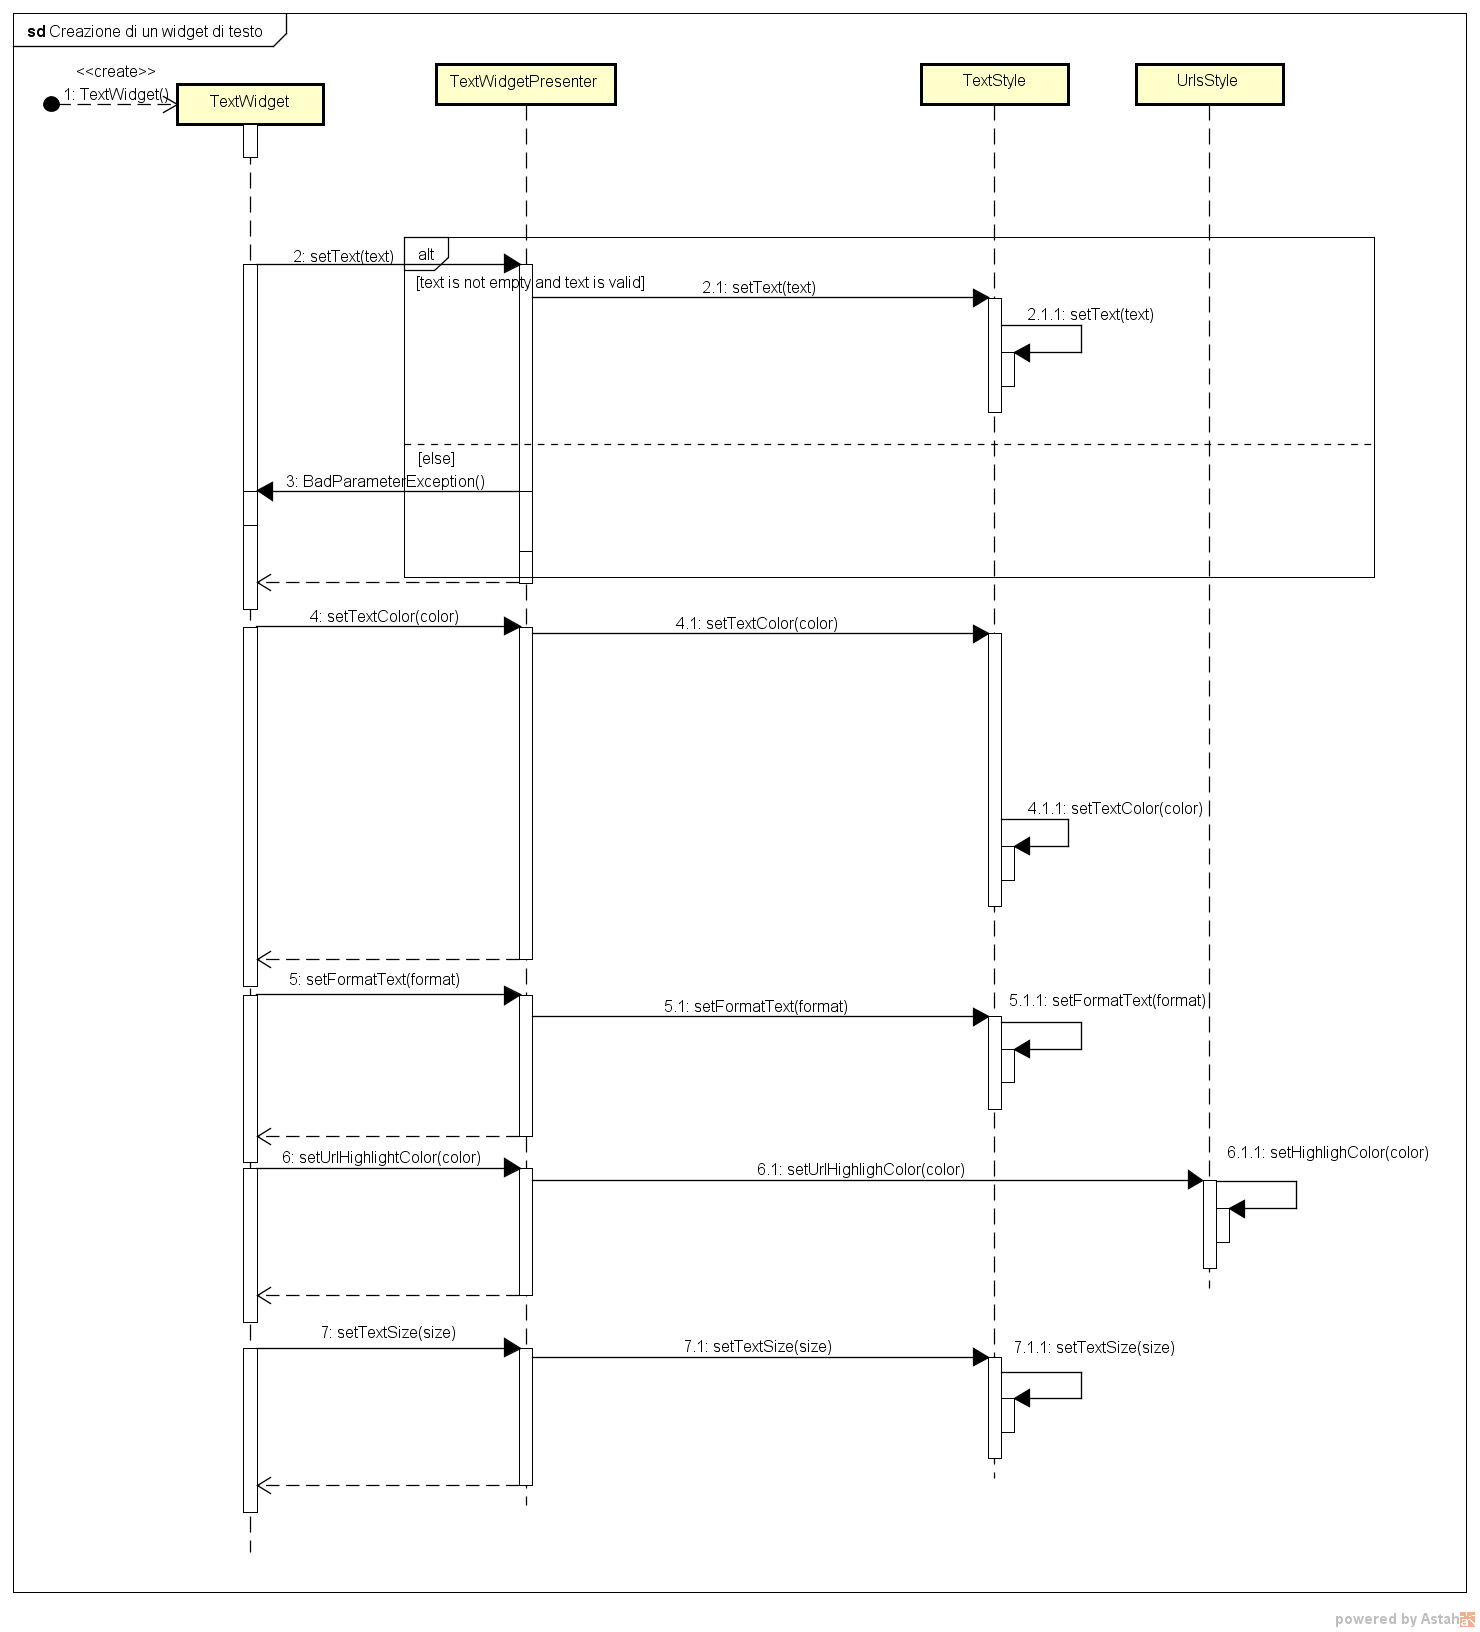
\includegraphics[width=16cm, height=14cm]{Sezioni/Diagrammi/SDK/Creazione di un widget di testo.png}
	\caption{Creazione di un widget di testo}
\end{figure}

Lo sviluppatore può creare un widget di tipo testo per aggiungerlo ad una sua ipotetica \termine{bolla}. Affinché non si verifichino errori il testo inserito nel widget deve essere valido, ovvero non deve contenere caratteri speciali se non quelli supportati dal tipo di codifica UTF-8 e non deve essere del testo vuoto. Se ciò dovesse capitare il metodo \texttt{setText} di \texttt{TextWidgetPresenter} lancerà un'eccezione di tipo \texttt{BadParameterException}. \\
Le frecce di ritorno dal \texttt{TextWidgetPresenter}  al \texttt{TextWidget} sono state inserite poiché il cambiamento dei dati sul \termine{Presenter} ha effetto anche sulla View. \\
Si noti, infine, che i metodi invocati da \texttt{TextWidget} vengono chiamati in quest'ordine dal suo costruttore senza parametri. Tali metodi possono anche essere chiamati singolarmente dallo sviluppatore secondo l'ordine che egli preferisce. Queste azioni non verranno ulteriormente descritte poiché ritenute ridondanti.

\newpage

\subsubsection{Creazione di un widget ChecklistItem}

\label{Creazione di un widget ChecklistItem}
\begin{figure}[H]
	\centering
	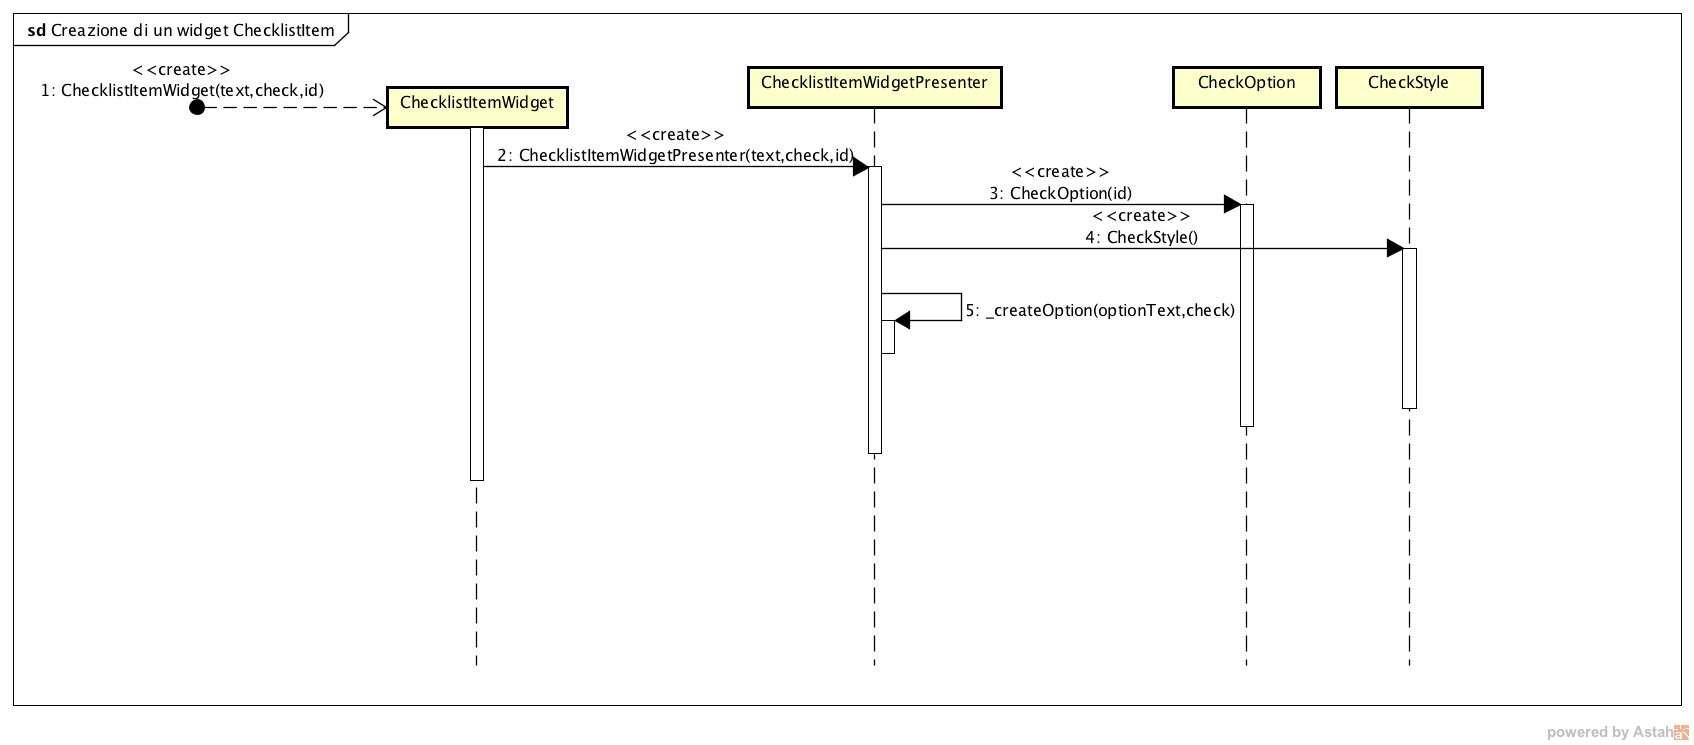
\includegraphics[width=16cm, height=14cm]{Sezioni/Diagrammi/SDK/Creazione di un widget ChecklistItem.png}
	\caption{Creazione di un widget ChecklistItem}
\end{figure}

Lo sviluppatore può creare un widget di tipo ChecklistItem per aggiungerlo ad una sua ipotetica \termine{bolla}. Al momento dell'invocazione del costruttore di ChecklistItemWidget verrà quindi creato un nuovo oggetto ChecklistItemWidget, che da il via alla costruzione di ChecklistItemWidgetPresenter, il quale a sua volta si occuperà della creazione di CheckOption e CheckStyle.\\
Una volta terminata l'operazione qui sopra descritta, verrà richiamato, da parte del presenter, il metodo privato \texttt{\_createOption} il quale terminerà la creazione degli elementi necessari alla visualizzazione del widget.
\newpage

\subsubsection{Creazione di un widget bottone}

\label{Creazione di un widget bottone}
\begin{figure}[H]
	\centering
	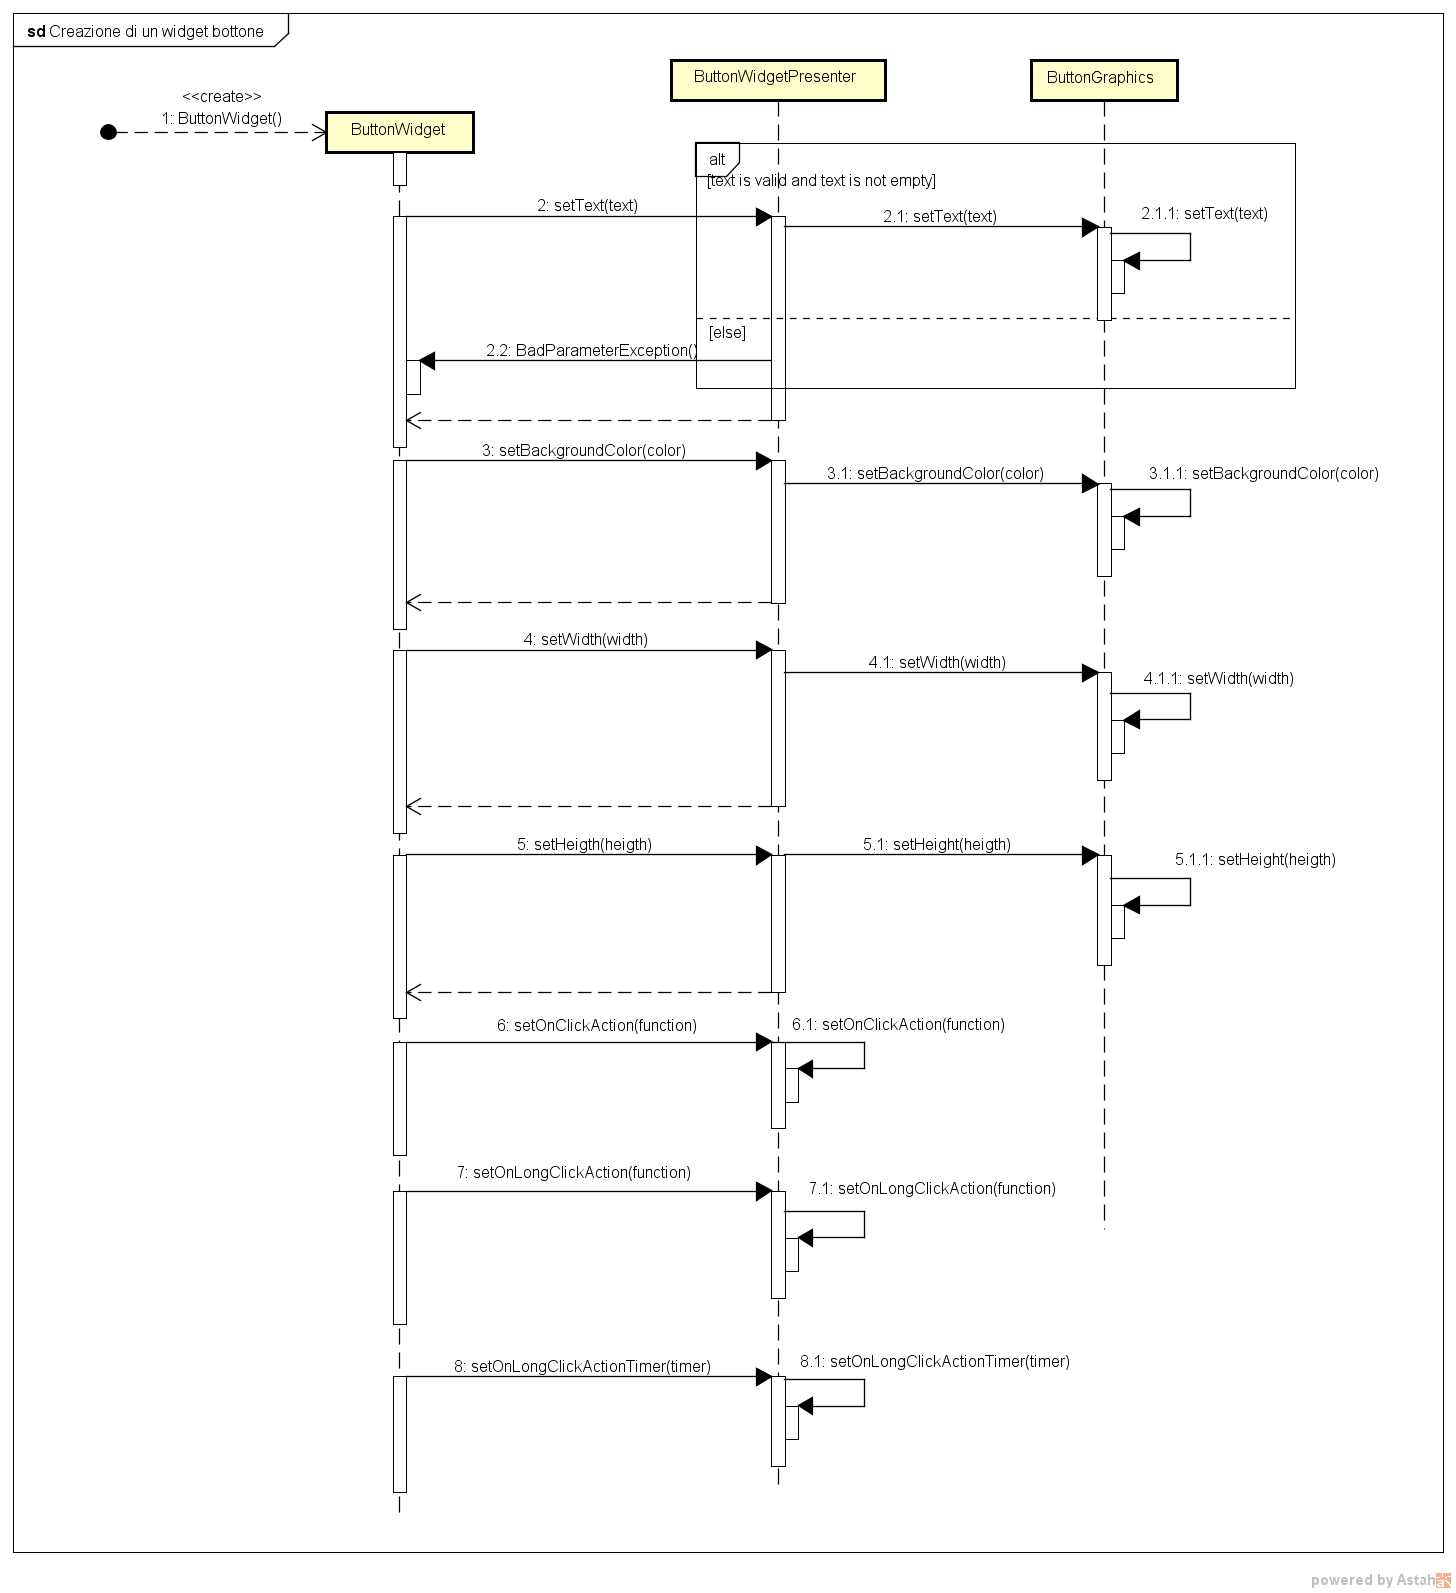
\includegraphics[width=16cm, height=14cm]{Sezioni/Diagrammi/SDK/Creazione di un widget bottone.png}
	\caption{Creazione di un widget bottone}
\end{figure}

Lo sviluppatore può creare un widget di tipo bottone per aggiungerlo ad una sua ipotetica \termine{bolla}. Se, durante la creazione del widget, il testo non dovesse essere impostato correttamente, il metodo \texttt{setText} di \texttt{ButtonWidgetPresenter} lancerà un'eccezione di tipo \texttt{BadParameterException}. \\
Le frecce di ritorno da \texttt{ButtonWidgetPresenter}  a \texttt{ButtonWidget} sono state inserite poiché il cambiamento dei dati sul \termine{Presenter} ha effetto anche sulla View. \\
Si noti, infine, che i metodi invocati da \texttt{ButtonWidget} vengono chiamati in quest'ordine dal suo costruttore senza parametri. Tali metodi possono anche essere chiamati singolarmente dallo sviluppatore secondo l'ordine che egli preferisce. Queste azioni non verranno ulteriormente descritte poiché ritenute ridondanti.

\newpage

\subsubsection{Creazione di un widget lista}

\label{Creazione di un widget lista}
\begin{figure}[H]
	\centering
	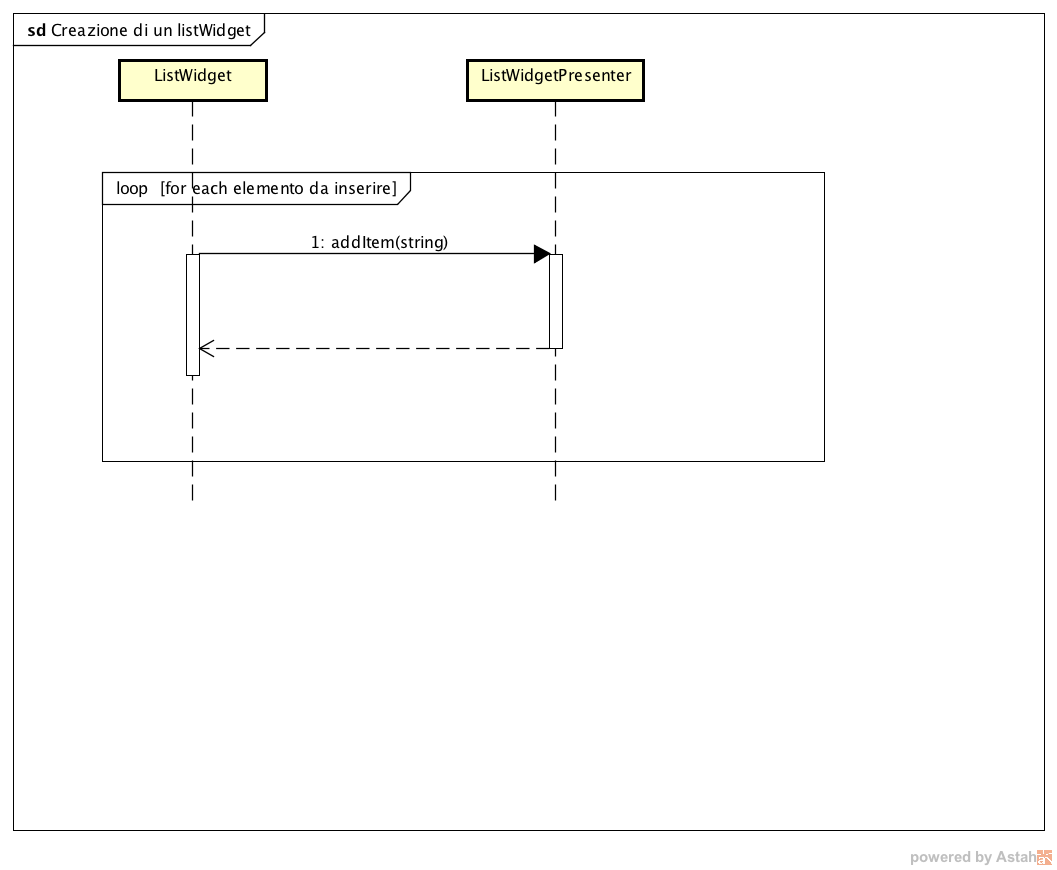
\includegraphics[width=16cm, height=14cm]{Sezioni/Diagrammi/SDK/Creazione di un listWidget.png}
	\caption{Creazione di un widget lista}
\end{figure}

Lo sviluppatore può creare un widget di tipo lista per aggiungerlo ad una sua ipotetica \termine{bolla}. Ogni elemento aggiunto logicamente dal presenter agisce anche sulla view. \\
L'azione compiuta per creare il widget può essere anche effettuata a posteriori della creazione del widget, questa però, essendo molto simile a quella appena descritta, viene omessa per ridondanza.

\newpage

\begin{comment}
\subsubsection{Creazione di una bolla aggiungendo un widget ChecklistItem}

\label{Creazione di una bolla aggiungendo un widget ChecklistItem}
\begin{figure}[H]
	\centering
	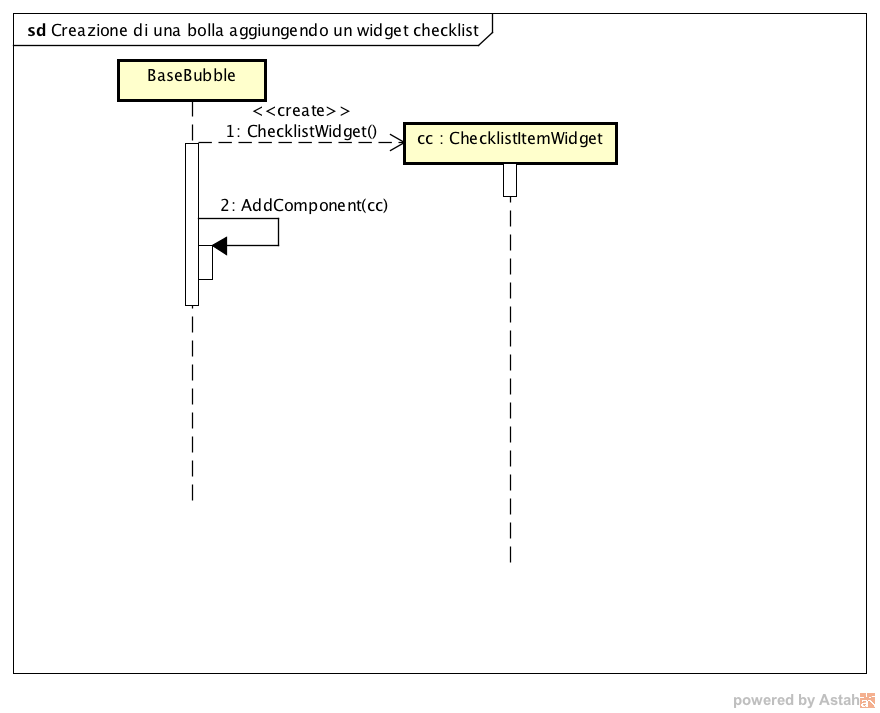
\includegraphics[width=16cm, height=14cm]{Sezioni/Diagrammi/SDK/Creazione di una bolla aggiungendo un widget checklist.png}
	\caption{Creazione di una bolla aggiungendo un widget ChecklistItem}
\end{figure}

Lo sviluppatore può aggiungere un widget alla \termine{bolla} appena creata. L'aggiunta dell'elemento avviene tramite il metodo \texttt{addComponent} che permette l'aggiunta sia di un layout che di un widget. Si noti che l'esempio è fatto con un widget specifico, ovvero il widget ChecklistItem, ma ciò vale per qualsiasi widget presente nell'\termine{SDK}. Gli altri esempi simili vengono, per questo motivo, omessi.

\newpage
\end{comment}

\subsubsection{Aggiunta ad una bolla di un Layout contenente due widget di testo}

\label{Aggiunta ad una bolla di un Layout contenente due widget di testo}
\begin{figure}[H]
	\centering
	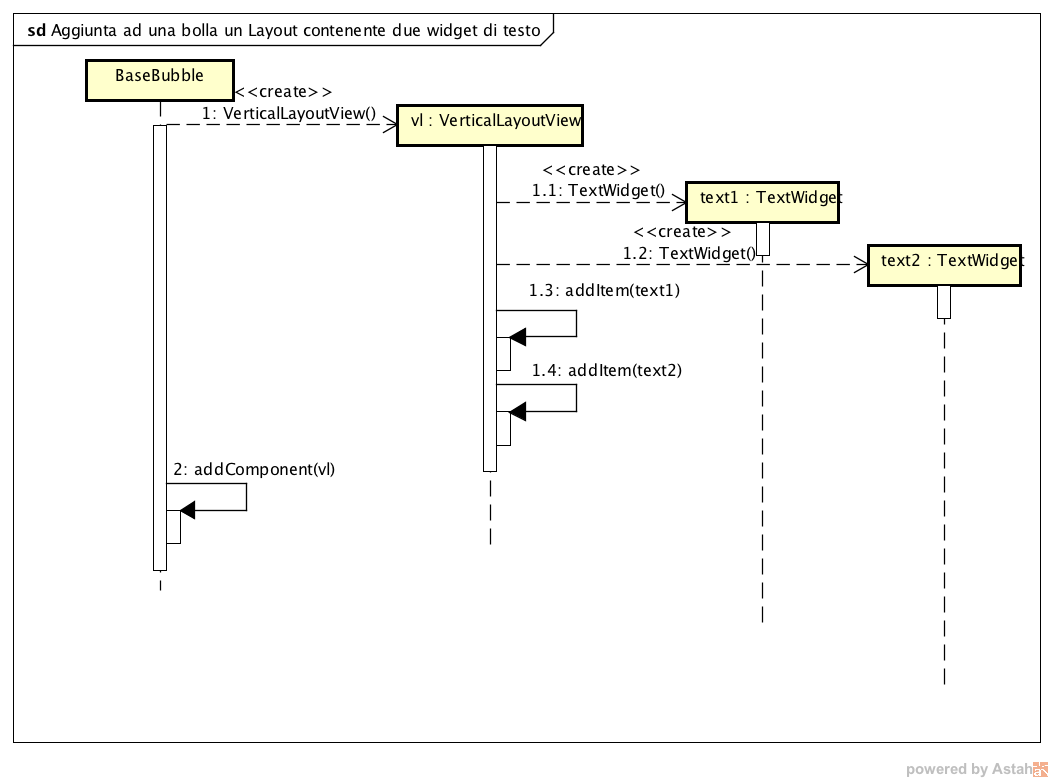
\includegraphics[width=16cm, height=14cm]{Sezioni/Diagrammi/SDK/Aggiunta ad una bolla un Layout contenente due widget di testo.png}
	\caption{Aggiunta ad una bolla di un Layout contenente due widget di testo}
	
\end{figure}
Lo sviluppatore può aggiungere un layout contenente dei widgets alla \termine{bolla}. Anche questo rappresenta solo un generico esempio di come si possa aggiungere un layout ad una \termine{bolla}. Gli altri esempi simili saranno dunque omessi. 

\newpage